\chapter{Scalar polynomials}


In this chapter, we introduce some basic theory regarding scalar polynomials%
\footnote{Polynomials were perhaps the first abstract mathematical object I encountered --- I distinctly remember grappling with the meaning of a variable \(x\), which is ``somehow a number but also not'', in the later years of elementary school. It's amazing, then, that the theory of polynomials of a single variable underlies so much of my PhD thesis.}
which will come in handy throughout the rest of this thesis.
A scalar polynomial of degree \( k \) is a function of the form 
\begin{equation*}
    x\mapsto c_0 + c_1 x + \cdots + c_k x^k,
%    ,\qquad 
%    c_0,c_1, \ldots, c_k\in \R.
\end{equation*}
where \( c_0, c_1, \ldots, c_k \) are fixed scalars.
Such a polynomial is naturally extended to matrices as
\begin{equation*}
    \vec{A} \mapsto c_0 \vec{I} + c_1 \vec{A} + \cdots + c_k \vec{A}^k
\end{equation*}
in a manner compatible with our definition of matrix functions.
Thus, matrix polynomials are intimately related to Krylov subspace methods.

%The precise relationship with Lanczos-based methods is discussed in \cref{sec:poly_insuff} where we provide more detail on our assertion that bounds based on best polynomial approximation on a single interval are often insufficient.


\section{Basic definitions}

Our discussion on quadrature centers around approximating distributions and integrals against distribution functions. 
Several examples of such functions are illustrated in \cref{fig:ch2_sample_dist}.

\begin{figure}[htb]
    \begin{center}
        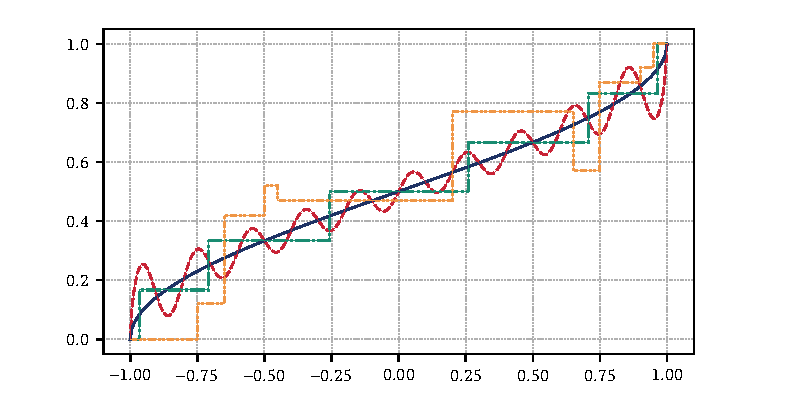
\includegraphics{imgs/ch2_sample_dist.pdf} 
    \end{center}
    \caption[Sample unit mass distribution functions.]{%
    Sample unit mass distribution functions.
    \hspace{.25em}\emph{Legend}:
    continuous increasing distribution function ({\protect\raisebox{0mm}{\protect
\includegraphics[]{imgs/legend/l1nm.pdf}}}),
    continuous distribution function which is not weakly-increasing ({\protect\raisebox{0mm}{\protect
\includegraphics[]{imgs/legend/l2nm.pdf}}}),
    discrete weakly-increasing distribution function ({\protect\raisebox{0mm}{\protect
\includegraphics[]{imgs/legend/l3nm.pdf}}}),
    discrete distribution function which is not weakly-increasing ({\protect\raisebox{0mm}{\protect
\includegraphics[]{imgs/legend/l4nm.pdf}}}).
    }
    \label{fig:ch2_sample_dist}
\end{figure}


\begin{definition}
A (signed) unit mass distribution function \( \Upsilon \) is a right continuous function \( \Upsilon:\R\to\R \) such that \( \lim_{x\to\infty} \Upsilon(x) = 1 \) and \( \lim_{x\to-\infty} \Upsilon(x) = 0 \).
If \( \Upsilon \) is also weakly increasing, we say it is a probability distribution function.
\end{definition}

\begin{remark}
    If \( \Upsilon \) is differentiable, then the derivative \( \d\Upsilon / \d{x} = \Upsilon' \) is the usual probability density function.
    Likewise, in the sense of distributions, \( \d\bOne[a \leq x] /\d{x} = \delta(x-a) \) where \( \delta(x-a) \) is a unit mass Dirac delta function centered at \( a \).
    Thus, if \( \Upsilon \) is piecewise constant, then \( \d\Upsilon/\d{x} \) can be expressed in terms of the sum of weighted Dirac delta functions, where a delta function is located at each discontinuity and weighted by the size of the corresponding jump.
\end{remark}

We now introduce several definitions which we will use throughout the next several chapters.
\begin{definition}
    Given a function \( f \) and distribution function \( \Upsilon \) we denote by 
        \( 
        \int_{a}^{b} f \,\d \Upsilon
        \) the standard Riemann--Stieltjes integral% defined by
        \begin{equation*}
            \int_a^b f \,\d \Upsilon
            := \lim_{\|P\|\to 0} \smop[r]{\sum_{i=0}^{p-1}} f(c_i) \big( \Upsilon(x^{(i+1)}) - \Upsilon(x^{(i)}) \big),
        \end{equation*}
        where \( P = \{ a = x^{(0)} < \cdots < x^{(p)} = b \} \) is a partition of \( [a,b] \), \( \| P \| = \max_i | x^{(i+1)} - x^{(i)}| \), and \( c_i \in [x_i,x_{i+1}] \).

    For notational clarity, we will often write 
    \(
    \int f \,\d \Upsilon
    \)
    in which case \( a,b \) can be taken as \( \pm \infty \).%\in \mathbb{R} \cup \{\pm \infty\} \) are understood to be such that \( \Upsilon \) is constant on \( (-\infty,a) \) and \( (b,\infty) \).
\end{definition}


\begin{definition}
    In the setting of the previous definition,
    \begin{equation*}
        \int_{a}^{b} f \, |\d \Upsilon|
        := \lim_{\|P\|\to 0} \smop[r]{\sum_{i=0}^{p-1}} f(c_i) \big| \Upsilon(x^{(i+1)}) - \Upsilon(x^{(i)}) \big|.
    \end{equation*}
\end{definition}

\begin{definition}
    Let \( \Upsilon \) be a (distribution) function.
The total variation (TV) of \( \Upsilon \), denoted \( \TV(\Upsilon) \), is defined by
\begin{equation*}
    \TV(\Upsilon) := \int |\d \Upsilon|.
\end{equation*}
\end{definition}
\begin{remark}
If \( \Psi \) is a weakly-increasing unit-mass distribution function, then \( \TV(\Psi) = 1 \). 
\end{remark}

To measure the similarity of two distribution functions, we will typically use the Wasserstein (earth mover) distance.
\begin{definition}
\label[definition]{def:wasserstein}
Let \( \Upsilon_1 \) and \( \Upsilon_2 \) be two probability distribution functions.
The Wasserstein distance between \( \Upsilon_1 \) and \( \Upsilon_2 \), denoted \( \W(\Upsilon_1,\Upsilon_2) \), is defined by
\begin{equation*}
    \W(\Upsilon_1,\Upsilon_2) 
    := \int | \Upsilon_1 - \Upsilon_2 | \,\d{x}.
\end{equation*}
\end{definition}

It is well known that the Wasserstein distance between two distribution functions has a dual form involving 1-Lipshitz functions. 
\begin{definition}
    We say that \( f\in \mathsf{Lip}(L,S) \) if \( |f(x) - f(y)| \leq L|x-y| \) for all \( x,y \in S \subseteq \R \).
\end{definition}

\begin{lemma}
\label[lemma]{thm:wasserstein_1lip}
    Suppose \( \Upsilon_1 \) and \( \Upsilon_2 \) are two probability distribution functions of bounded total variation each constant on \( (-\infty,a) \) and \( (b,\infty) \).
Then,
\begin{equation*}
    \W(\Upsilon_1,\Upsilon_2) = \sup \left\{ \int f \d \big( \Upsilon_1 - \Upsilon_2\big) : f\in\textup{\textsf{Lip}}(1,[a,b]) \right\}.
\end{equation*}
\end{lemma}
\begin{remark}
    In some situations, other metrics may be more meaningful. 
    For instance, if it is important for two distribution functions to agree to very high precision in a certain region, but only to moderate accuracy in others, then the Wasserstein distance may be unsuitable.
\end{remark}


\section{Orthogonal polynomials}
\label{sec:OP}


Throughout this thesis, \( \mu \) will be a non-negative unit mass distribution function. 
Associated with \( \mu \) is the inner product \( \langle \cdot, \cdot \rangle_\mu \) defined by
\label{def:mu}
\begin{equation}
    \label{eqn:mu_ip}
    \langle f, g\rangle_\mu\: := \int fg \,\d\mu.
\end{equation}

The set of \( \mu \)-square-integrable functions forms a Hilbert space with respect to this inner product, so we may hope to find an orthonormal basis \( \{ p_i \}_{i=0}^{\infty} \) of polynomials with \( \deg(p_i) = i \). \label{def:OP}
Such a basis is easily produced by a simple modification of the Gram-Schmidt algorithm which results in a naive implementation of the so-called Stieltjes algorithm.
An implementation is described in \cref{alg:stieltjes_naive}.

\begin{labelalgorithm}[H]{stieltjes_naive}{Stieltjes}{Stieltjes algorithm (naive)}
\begin{algorithmic}[1]
    \Procedure{\thealgorithmname}{$\mu,k$}
    \State \( p_0 = 1 \)
    \For {\( i=0,1,\ldots, k-1 \)}
        \State \( \tilde{p}_{i+1} = x p_i \)
        \State \( \hat{p}_{i+1} = \tilde{p}_{i+1} - \big(\langle p_0, \tilde{p}_{i+1} \rangle_\mu\: p_0  +  \cdots + \langle p_{i}, \tilde{p}_{i+1} \rangle_\mu\: p_i \big) \)
        \State \( p_{i+1} = \hat{p}_{i+1} / \| \hat{p}_{i+1} \|_\mu\: \)
    \EndFor
    \State \Return \( \{ p_i \}_{i=0}^{k} \) 
\EndProcedure
\end{algorithmic}
\end{labelalgorithm}

Note that the polynomials satisfy, for all \( i\geq 0 \),
\begin{equation}
    \label{eqn:all_term_recurrence}
    x p_i = \| \hat{p}_{i+1} \|_\mu\: p_{i+1} + \langle p_0, \tilde{p}_{i+1} \rangle_\mu\: p_0  +  \cdots + \langle p_{i}, \tilde{p}_{i+1} \rangle_\mu\: p_i.
\end{equation}
This can be written in matrix form as
\begin{equation*}
x\, [p_0, p_1, \ldots ] = [p_0, p_1, \ldots ] \vec{H},
\end{equation*}
where \( [p_0, p_1, \ldots ] \) is a \emph{quasi-matrix} whose columns are the polynomials \( \{ p_i \}_{i=0}^{\infty} \) and \( \vec{H} \) is a semi-infinite upper-Hessenberg matrix.
Moreover, for all \( i,j \geq 0 \),
\begin{equation*}
    [\vec{H}]_{i,j} = \langle p_i, x p_j \rangle_\mu  = \langle p_j, x p_i \rangle_\mu = [\vec{H}]_{j,i};
\end{equation*}
that is, \( \vec{H} \) is symmetric. 
Since, by construction, \( \vec{H} \) is upper-Hessenberg, this implies that \( \vec{H} \) is symmetric tridiagonal!

Therefore, for all \( i\geq0 \), \cref{eqn:all_term_recurrence} becomes the symmetric three-term recurrence
\begin{equation}
    \label{eqn:poly_three_term}
    x p_i =  \beta_{i-1} p_{i-1} + \alpha_i p_i + \beta_{i} p_{i+1}
\end{equation}
with initial conditions \( p_0 = 1 \), \( p_{-1} = 0 \), and \( \beta_{-1} = 0 \), where \( \{ \alpha_i \}_{i\geq0} \) and \( \{ \beta_i \}_{i\geq 0} \) are chosen to enforce orthogonality.
In particular, \cref{alg:stieltjes_naive} can be modified to take advantage of this short-recurrence, resulting in the standard implementation of the Stieltjes algorithm, \cref{alg:stieltjes}.
In the case that \( \beta_i = 0 \), the algorithm should be terminated as the dimension of Krylov subspaces does not continue to grow.

\begin{labelalgorithm}[htb]{stieltjes}{Stieltjes}{Stieltjes algorithm}
\begin{algorithmic}[1]
    \Procedure{\thealgorithmname}{$\mu,k$}
    \State \( p_0 = 1 \)
    \For {\( i=0,1,\ldots, k-1 \)}
        \State \( \tilde{p}_{i+1} = x p_i \)
        \State \( \alpha_i = \langle p_i, \tilde{p}_{i+1} \rangle_\mu \)
        \State \( \hat{p}_{i+1} = \tilde{p}_{i+1} - \alpha_i p_i \)
        \State \( \beta_{i} = \| \hat{p}_{i+1} \|_\mu\: \) 
        \State \( p_{i+1} = \hat{p}_{i+1} / \beta_i \)
    \EndFor
    \State \Return \( \{ p_i \}_{i=0}^{k} \), \( \{ \alpha_i \}_{i=0}^{k-1} \), \( \{\beta_i\}_{i=0}^{k-1} \) 
\EndProcedure
\end{algorithmic}
\end{labelalgorithm}

\begin{definition}
    \label{def:jacobi}
    The, possibly semi-infinite, tridiagonal matrix \( \vec{M} = \vec{M}(\mu) \) giving the three-term recurrence coefficients for the orthogonal polynomials of \( \mu \) is called the Jacobi matrix corresponding to \( \mu \). 
    Unless specified otherwise, the coefficients are 
    \begin{equation*}
    \vec{M} = 
    \begin{bmatrix}
        \alpha_0 & \beta_0 \\
        \beta_0 & \alpha_1 & \beta_1 & \phantom{\ddots}\\
        &\beta_1 & \alpha_2 & \ddots \\
        &&\ddots & \ddots \\
    \end{bmatrix}.
\end{equation*}
%and for a distribution \( \nu \), different from \( \mu \), we will denote the corresponding Jacobi matrix by \( \vec{M}(\nu) \).   
\end{definition}

An important property of a distribution function \( \Upsilon \) are it's polynomial moments.
We are particularly interested in those induced by \( \mu \).
\begin{definition}
\label{def:modified_moments}
For each \( i \geq 0 \), the modified moments of \( \Upsilon \) (with respect to \( \mu \)) are 
\begin{equation*}
    m_i = m_i(\Upsilon,\mu) := \int p_i \,\d\Upsilon.
\end{equation*}
If \( m_0, \ldots, m_{s} < \infty \), we say \( \Upsilon \) has finite moments through degree \( s \).
\end{definition}
 

Jacobi matrices have many interesting properties, several of which we review here.

\begin{lemma}
    The upper-leftmost \( k\times k \) submatrix of a Jacobi matrix is entirely determined by the moments through degree \( 2k-1 \) of the associated distribution function.
\end{lemma}

\begin{proof}
    This is a direct consequence of the fact that the \( k \)-point (degree \( 2k-1 \)) Gaussian quadrature rule for a distribution function can be determined from the upper-leftmost \( k\times k \) submatrix of the associated Jacobi matrix.
    This argument will be made whole in \cref{sec:gq}.
\end{proof}

\begin{lemma}
    \label{thm:jacobi_eigen}
    Denote the zeros of \( p_{k} \) by \( \{ \theta_j^{(k)} \}_{j=0}^{k-1} \).
Then, for any \( j=0,1,\ldots, k-1 \),
\begin{equation*}
    \label{eqn:jacobi_evec}
    \big[ p_0(\theta_{j}^{(k)}), p_1(\theta_{j}^{(k)}), \ldots, p_{k-1}(\theta_{j}^{(k)}) \big]^\cT
\end{equation*}
is an eigenvector of \( [\vec{M}]_{:k,:k} \) with eigenvalue \( \theta_{j}^{(k)} \).
Moreover, all eigenvectors are obtained in this way.
\end{lemma}

\begin{proof}
    In matrix form, \cref{eqn:poly_three_term} becomes
    \begin{equation*}
        x\, [p_0, p_1, \ldots, p_{k-1} ] = [p_0, p_1, \ldots, p_{k-1}] \vec{M} + \beta_{k-1} p_{k} \vec{e}_{k-1}^\rT.
    \end{equation*}
    Evaluating each side of the above equality at \( \theta_j^{(k)} \) gives the first part of the result.

    To show all eigenvectors are obtained in this way, it suffices to show that \( \{ \theta_j^{(k)} \}_{0\leq j<k} \) are distinct.
    Let \( \{ t_j \}_{j=0}^{k'-1} \) be the points at which \( p_{k} \) changes signs. 
    Then, 
    \begin{equation*}
        \int p_k {\prod_{j=0}^{k'-1}} (x-t_j) \,\d \mu \neq 0
    \end{equation*}
    since the integrand does not change signs.
    This implies \( k' = k \) since \( p_k \) is orthogonal to all polynomials of lower degree.
\end{proof}





\subsection{Chebyshev polynomials}

Owing to the deep connection between Chebyshev polynomials and approximation theory \cite{trefethen_19}, one particularly important choice of \( \mu \) is the distribution function corresponding to the Chebyshev polynomials of the first kind. 
We will often treat this case with special care.
%While we treat the case of the Chebyshev polynomials of the first kind, similar results can usually be expected for other classical orthogonal polynomials.
\begin{definition}
    \label{def:muT}
    The Chebyshev distribution function of the first kind, \( \mu_{a,b}^T : [a,b] \to [0,1] \), is defined as
    \begin{equation*}
        \mu_{a,b}^T 
        := \frac{1}{2} + \frac{1}{\pi}\arcsin\left(\frac{2}{b-a}x - \frac{b+a}{b-a}\right).
    \end{equation*}
    Thus, for \( x\in[a,b] \),
    \begin{equation*}
        \frac{\d\mu_{a,b}^T}{\d{x}}
        = \frac{2}{\pi(b-a)} \Big(1-\big(\frac{2}{b-a}x - \frac{b+a}{b-a}\big)^2\Big)^{-1/2}.
    \end{equation*}    
\end{definition}

\begin{definition}
    The Chebyshev polynomials of the first kind, denoted \( \{ T_i \}_{i=0}^{\infty} \), are defined by the recurrence \( T_0 = 1 \), \( T_1 = x \), and, for all \( i \geq 1 \),
    \begin{equation*}
        T_{i+1} := 2 x T_i - T_{i-1}.
    \end{equation*}
\end{definition}

    It can be verified that the orthogonal polynomials \( \{p_i\}_{i=0}^{\infty} \) with respect to \( \mu_{a,b}^T \) are given by \( p_0 = T_0 = 1 \) and, for all \( i \geq 1 \),
    \begin{equation*}
        p_i = \sqrt{2} T_i \left( \frac{2}{b-a} x + \frac{b+a}{b-a} \right).
    \end{equation*}

    Therefore, the Jacobi matrix \( \vec{M}( \mu_{a,b}^T ) \) has diagonal and off diagonals entries given by
    \begin{equation*}
        \left[ \frac{a+b}{2}, \frac{a+b}{2}, \ldots \right]
        \quad\text{and}\quad
        \left[ \frac{b-a}{2\sqrt{2}} , \frac{b-a}{4}, \frac{b-a}{4} , \ldots  \right],
    \end{equation*}
    respectively.



\section{Polynomial approximations and bounds}
\label{sec:uniform_poly_bounds}

As noted in the introduction, we use the notation \( \ff{f}{s} \) to denote a degree \( s \) polynomial obtained from \( f \) by some algorithm parameterized by \( \circ \).
In particular, we will make the following definitions.
\begin{definition}
    \label{def:fffs}
    Given a non-negative unit mass distribution function \( \mu \) with degree \( s+1 \) orthogonal polynomial \( p_{s+1} \) we define,
    \begin{equation*}
        \ff{f}{s} := 
        \begin{cases}
            \circ = \text{i} & \text{degree $s$ interpolant to \( f \) at roots of $p_{s+1}$} \\
            \circ = \text{a} & \text{degree $s$ truncated series for \( f \) in \( \langle \cdot, \cdot \rangle_\mu \)} \\
%            \circ = \text{d-i} & \text{damped degree $s$ interpolant to \( f \) at roots of $p_{s+1}$} \\
%            \circ = \text{d-a} & \text{damped degree $s$ approximation to \( f \) in \( \langle \cdot, \cdot \rangle_\mu \)} \\
        \end{cases}
    \end{equation*}.
\end{definition}

The damped projection \( \ff[d-a]{f}{s} \) and damped interpolant \( \ff[d-i]{f}{s} \) are respectively obtained by scaling each of the coefficients of \( \ff[a]{f}{s} \) and \( \ff[i]{f}{s} \), when represented as a linear combination of the orthogonal polynomials \( \{ p_i \}_{i=0}^{s} \), by constants \( \rho_i \) for each \( i = 0,1,\ldots, s\).
\begin{definition}
\label{def:damping}
    Write \( \ff{f}{s} \) in a polynomial series with respect to \( \langle \cdot, \cdot \rangle_\mu \)\,; i.e. as
    \begin{equation*}
        \ff{f}{s} = \: \smop{\sum_{i=0}^{s}} c_i p_i.
    \end{equation*}
    Then, given damping coefficients \( \{ \rho_i \}_{i=0}^{s} \) with \( 0\leq \rho_i \leq 1 \) for all \( i \),
    \begin{equation*}
        \ff[d-$\circ$]{f}{s} := \: \smop{\sum_{i=0}^{s}} \rho_i c_i p_i.
    \end{equation*}
\end{definition}



We now review several classical results from approximation theory which we will use throughout this thesis.
These are constructive bounds for the case \( \mu = \mu_{-1,1}^T \) which provide upper bounds for the quality of the \emph{best} polynomial approximation to \( f \).
In fact, both  \( \ff[a]{f}{s} \) and \( \ff[i]{f}{s} \) provide nearly optimal approximations in many settings \cite{trefethen_19}.

A full treatment requires at least a textbook, and we refer readers to \cite{trefethen_19} for an excellent such book.
The following theorems are summarized from Theorems 7.2 and 8.2 in \cite{trefethen_19}.

\begin{definition}
    We say that \( f\in \mathsf{BV}(d,V,S) \) if, on \( S\subseteq \R \), \( f \) is \( d \) times differentiable, its derivatives through \( f^{(d-1)} \) are absolutely continuous, and the \( d \)-th derivative \( f^{(d)} \) has total variation bounded above by some constant \( V \) on \( S \).
\end{definition}


\begin{definition}
    For \( \rho \geq 1 \) the Bernstein ellipse \( E_\rho(a,b) \) is the ellipse centered at \( \frac{a+b}{2} \) with semi-axis lengths \( \frac{b-a}{2} \frac{1}{2} (\rho + \rho^{-1}) \) and \( \frac{b-a}{2}\frac{1}{2} (\rho+\rho^{-1}) \) along the real and imaginary directions; i.e
    \begin{equation*}
        E_\rho(a,b) = \left\{ z \in\mathbb{C} : z = \frac{b-a}{2} \frac{1}{2} (u + u^{-1}) + \frac{a+b}{2}, \: u = \rho \exp(i\theta), \: \theta\in[0,2\pi) \right\}. 
    \end{equation*}
\end{definition}


\begin{definition}
    We say that \( f\in \mathsf{Anl}(\rho,M,[a,b]) \) if \( f \) is analytic on the region enclosed by \( E_\rho(a,b) \) where it satisfies \( |f(x)|\leq M \).
\end{definition}

\begin{theorem}
    \label{thm:bv_cheb}
    For an integer \( d \geq 0 \), suppose \( f \) is \( d \) times differentiable, its derivatives through \( f^{(d-1)} \) are absolutely continuous, and the \( d \)-th derivative \( f^{(d)} \) has total variation bounded above by some constant \( V \) on \( [-1,-1] \); i.e., suppose \( f \in \textup{\textsf{BV}}(d,V,[-1,1]) \).
    Then, with \( \mu = \mu_{-1,1}^T \), for any \( s > d \), 
    \begin{equation*}
        \| f - \ff[a]{f}{s} \|_{[-1,1]} \leq \frac{2 V}{\pi d(s-d)^d}
        ,\qquad
        \| f - \ff[i]{f}{s} \|_{[-1,1]} \leq \frac{4 V}{\pi d(s-d)^d}.
    \end{equation*}
\end{theorem}

\begin{theorem}
    \label{thm:analytic_cheb}
    Suppose \( f \) is analytic on the region enclosed by the Bernstein ellipse \( E_\rho(-1,1) \) where it satisfies \( \|f\|_{E_{\rho(-1,1)}} \leq M \); i.e., suppose \( f\in \textup{\textsf{Anl}}(\rho,M,[-1,1]) \).
    %Let a function \( f \) analytic in \( [-1,1] \) be analytically continuance to the open Bernstein ellipse \( E_{\rho} \), where it satisfies \( |f(z)| \leq M \) for some \( M \).
    Then, with \( \mu = \mu_{-1,1}^T \), for any \( s \geq 0 \), 
    \begin{equation*}
        \| f - \ff[a]{f}{s} \|_{[-1,1]} \leq \frac{2 M \rho^{-k}}{\rho - 1}
        ,\qquad
        \| f - \ff[i]{f}{s} \|_{[-1.1]} \leq \frac{4 M \rho^{-k}}{\rho - 1}.
    \end{equation*}
\end{theorem}

\begin{lemma}
    \label[lemma]{thm:cheb_rates}
    Set \( c_{\textup{i}} = 2 \) and \( c_{\textup{a}} = 1 \).
    Then, for \( \circ \in \{ \textup{i}, \textup{a} \} \), \( \| f - \ff[]{f}{s} \|_\infty < \epsilon / 2 \) provided
        \begin{equation*}
        s \geq 
         \begin{cases}
             \frac{1}{\ln(\rho)} \ln \left( \frac{4 c_\circ M}{\rho-1} \right) + \frac{1}{\ln(\rho)} \ln \left( \varepsilon^{-1} \right) & f \in \mathsf{Anl}(\rho,M,[a,b]), \\
             d + \left( \frac{4 c_\circ V}{\pi d} \right)^{1/d} \varepsilon^{-1/d} & f \in \mathsf{BV}(d,V,[a,b]) .
        \end{cases}   
        \end{equation*}
\end{lemma}
\begin{proof}
    Define \( \tilde{f} : \R\to\R\) by \( \tilde{f}(x) = f( \frac{b-a}{2} x + \frac{a+b}{2} ) \).
    Then we have that,
    \begin{equation*}
        \min_{\deg(p) \leq s} \| f - p \|_{[a,b]}
        = \min_{\deg(p) \leq s} \| \tilde{f} - p \|_{[-1,1]}.
    \end{equation*}
    
    Note that if \( f\in \mathsf{Anl}(\rho,M,[a,b]) \) then \( \tilde{f} \in \mathsf{Anl}(\rho,M,[-1,1]) \) and if \( f\in \mathsf{BV}(d,V,[a,b]) \) then \( \tilde{f} \in \mathsf{BV}(d,V,[-1,1]) \).

The result then follows by setting the upper bounds in \cref{thm:bv_cheb,thm:analytic_cheb} to \( \epsilon/2 \) and solving for \( s \).
\end{proof}

Next, we consider polynomial approximations to 1-Lipshitz functions.
Note that there exist 1-Lipshitz functions whose derivatives are not of bounded variation. 
Therefore we cannot simply use \cref{thm:bv_cheb}.
Fortunately, the best approximation of differentiable functions is well studied. 
In particular, we have the following theorem due to Jackson; see \cite[Section 87]{achieser_92} and \cite[Section 6]{cheney_00} for details.
\begin{theorem} % see also cheney ch 4 sec 6
\label{thm:jackson}
    Suppose \( f \) is 1-Lipshitz on \( [-1,1] \); i.e., suppose that \( f \in \textup{\textsf{Lip}}(1,[-1,1]) \).
Then,
\begin{equation*}
    \min_{\deg(p) \leq s} \| f - p \|_{[-1,1]} \leq \frac{\pi}{2} (s+1)^{-1}.
\end{equation*}
\end{theorem}
In fact, the constant \( \pi/2 \) is the best possible under the stated conditions.

While the ``vanilla'' Chebyshev projection and interpolation do not attain this rate for all 1-Lipshitz functions, we can constructively obtain polynomial approximations which do attain this rate by damping.
\begin{definition}
\label{def:jackson_coeffs}
For \( i=0,1,\ldots, s \), the degree \( s \) Jackson's damping coefficients are
\begin{equation*}
    \rho_{i}^{J}
    = \frac{(s-i+2)\cos \left( \frac{i \pi}{s+2} \right) + \sin \left( \frac{i \pi}{s+2} \right)\cot \left( \frac{\pi}{s+2} \right)}{s+2}.
\end{equation*}
\end{definition}
The damped projection and interpolant then satisfy a similar bound to \cref{thm:jackson}.
\begin{restatable}{theorem}{dampedcheb}
    \label{thm:damped_cheb}
    Suppose \( f \in \textup{\textsf{Lip}}(1,[-1,1]) \), \( \mu  = \mu_{-1,1}^T \), and we use Jackson's damping coefficients as in \cref{def:jackson_coeffs}.
    Then for \( \circ \in \{ \textup{d-i}, \textup{d-a} \} \),
    \begin{equation*}
        \| f - \ff[]{f}{s} \|_{[-1,1]} \leq \frac{\pi^2}{2} (s+2)^{-1}.
    \end{equation*}
\end{restatable}
We provide a proof of this statement in \cref{sec:damped_cheb}.
While our proof is based closely on \cite{rivlin_81}, the exact constant we obtain is sharper than other bounds we know of for the quality of the damped projection \( \ff[d-a]{f}{s} \).
Moreover, our version of the proof works for the damped interpolant \( \ff[d-i]{f}{s} \). 
We were unable to find a similar result in the literature, although we suspect such a result is known.
%We remark that it is somewhat curious that the bound for the damped projection and interpolant have the same constant; indeed most bounds for the Chebyshev inter


\begin{subappendices}
\section{Proof of Jackson's theorem}
\label{sec:damped_cheb}

In this section we prove \cref{thm:damped_cheb}.
%\dampedcheb*
We follow Chapter 1 of \cite{rivlin_81} closely, starting with trigonometric polynomials on \( [-\pi,\pi] \) and then mapping to algebraic polynomials on \( [-1,1] \).
Throughout this section we maintain the notation of \cite{rivlin_81}, so the constants in this section do not necessarily have the same meaning as the rest of the paper.
In particular, \( n \) is the degree of the trigonometric polynomials used.



Given \( g:\R\to\R \), 1-Lipshitz and \( 2\pi \)-periodic, for \( \circ \in \{ \textup{i}, \textup{a} \} \), define
\begin{equation*}
    s_n^\circ(\theta) 
    := \frac{a_0^\circ}{2} 
    + \smop{\sum_{k=1}^{n}} \left( a_k^\circ \cos(k\theta) + b_k^\circ \sin(k\theta) \right)
\end{equation*}
where, for \( k=0,1,\ldots, n \)
\begin{equation*}
    a_k^\circ := \frac{1}{\pi}\int_{-\pi}^{\pi^-} g(\phi) \cos(k\phi) M_n^\circ(\phi) \,\d\phi
    ,\qquad
    b_k^\circ := \frac{1}{\pi}\int_{-\pi}^{\pi^-} g(\phi) \sin(k\phi) M_n^\circ(\phi) \,\d\phi.
\end{equation*}
Here \( M_n^{\textup{a}}(\phi) := 1 \) and 
\begin{equation*}
    M_n^{\textup{i}}(\phi) 
    :=  \frac{\pi}{n} \sum_{i\in\mathbb{Z}}\delta(\phi-\phi_i)
    ,\qquad 
    \phi_i 
    := \frac{2\pi(i-1/2)}{2n} - \pi
\end{equation*}
where \( \delta(\phi) \) is a Dirac delta distribution centered at zero.
Thus, \( s_n^\textup{a} \) is the truncation of the Fourier series of \( g \) while \( s_n^{\textup{i}} \) is the interpolant to \( g \) at the equally spaced nodes \( \{ \phi_i \}_{i-0}^{2n} \).

\begin{remark}
    Note that \( \int_{-\pi}^{\pi^-} \) means an integral over \( [-\pi,\pi) \); i.e. the upper endpoint of integration is excluded. 
    This is important for integrals involving \( M_n^{\textup{i}} \) which can have nonzero integral at a single point.
\end{remark}


Finally, define the damped interpolant/approximant
\begin{equation*}
    q_n^\circ(\theta) 
    := \frac{a^\circ_0}{2} + \smop{\sum_{k=1}^{n}} \rho_k \left( a_k^\circ \cos(k \theta) + b_k^\circ \sin(k\theta) \right)
\end{equation*}
where the damping coefficients \( \{ \rho_{k} \}_{k=1}^{n} \) are arbitrary real numbers.
Our aim is to bound \( \| q_n^\circ - g \|_{[-\pi,\pi]} \).

\begin{lemma}
    \label[lemma]{thm:Dn_zero}
    For all \( k=0,1,\ldots, n \),
    \begin{equation*}
        \frac{1}{\pi} \int_{-\pi}^{\pi^-} \cos(k \phi) M_n^\circ(\phi) \,\d\phi
        = \begin{cases}
            2 & k = 0 \\%\in 4n\mathbb{Z} \\
            0 & k \in 1,2,\ldots, n
        \end{cases}
    \end{equation*}
    and
    \begin{equation*}
        \frac{1}{\pi} \int_{-\pi}^{\pi^-} \sin(k x) M_n^\circ(\phi) \,\d\phi
        = 0.
    \end{equation*}
\end{lemma}

\begin{proof} 
    Clearly \( \frac{1}{\pi} \int_{-\pi}^{\pi^-} \cos(0 \phi) M_n^{\textup{a}} \d\phi = 2 \), and for \( k > 0 \), we have,
    \begin{equation*}
        \frac{1}{\pi} \int_{-\pi}^{\pi^-} \cos(k\phi) M_n^{\textup{a}}(\phi) \,\d\phi
%        = \frac{\sin(-k\pi) - \sin(k\pi)}{k \pi} 
        = 0.
    \end{equation*}
    By definition, 
    \begin{equation*}
        \frac{1}{\pi} \int_{-\pi}^{\pi^-} \cos(k\phi) M_n^{\textup{i}}(\phi) \,\d\phi
        = \frac{1}{n} \smop{\sum_{j=1}^{2n}} \cos(k \phi_j)
        = \frac{1}{n} \operatorname{Re} \smop{\sum_{j=1}^{2n}} \exp( \ii k \phi_j).
    \end{equation*}
    The case for \( k=0 \) is clear.
    Assume \( k > 0 \).
    Then, using that \( \phi_j = \frac{\pi}{n}(j-\frac{1}{2}) - \pi \) we have
    \begin{equation*}
        \frac{1}{n} \operatorname{Re} \smop{\sum_{j=1}^{2n}} \exp( \ii k \phi_j) 
        = \frac{1}{n} \operatorname{Re}\left[ \exp \left(\ii k\left(\frac{\pi}{2n}- \pi\right) \right) \smop{\sum_{j=0}^{2n-1}} \exp \left( \ii \frac{k\pi}{n} j \right) \right].
    \end{equation*}
    The result follows by observing that 
    \begin{equation*}
        \smop{\sum_{j=0}^{2n-1}} \exp\left( \ii \frac{k \pi}{n} j \right) 
        =  \frac{\exp(2\ii k \pi)-1}{\exp(\ii k \pi/n) - 1} 
        = 0.
    \end{equation*}
    Finally, since \( \sin(k\phi) \) is odd and \( M_n^\circ \) is symmetric about zero, the corresponding integrals are zero.
\end{proof}


We now introduce a generalized version of \cite[Lemma 1.4]{rivlin_81}.
\begin{lemma}
    Define
    \begin{equation*}
        u_n(\phi) := \frac{1}{2} + \smop{\sum_{k=1}^{n}} \rho_{k} \cos(k\phi).
    \end{equation*} 
    Then,
    \begin{equation*}
        q_n^\circ(\theta) = \frac{1}{\pi} \int_{-\pi}^{\pi^-}g(\phi+\theta) u_n(\phi) M_n^\circ(\phi+\theta) \,\d\phi.
    \end{equation*}
\end{lemma}

\begin{proof}
    First, note that
    \begin{align*}
        \pi q_n^\circ(\theta)
        &= \frac{1}{2} \bigg( \int_{-\pi}^{\pi^-} g(\phi) M_n^\circ(\phi) \,\d\phi  \bigg) 
        + \smop{\sum_{k=1}^{n}} \rho_k 
        \bigg( 
        \bigg( \int_{-\pi}^{\pi^-} g(\phi) \cos(k\phi)  M_n^\circ(\phi) \,\d\phi \bigg) \cos(k\theta)
        \\&\hspace{4em} + \bigg( \int_{-\pi}^{\pi^-} g(\phi) \sin(k\phi)  M_n^\circ(\phi) \,\d\phi \bigg) \sin(k\theta)
        \bigg)
        \\&= \int_{-\pi}^{\pi^-} g(\phi) \bigg( \frac{1}{2} + \smop{\sum_{k=1}^{n}} \rho_{k}( \cos(k\phi) \cos(k\theta) + \sin(k\phi) \sin(k\theta)) \bigg) M_n^\circ(\phi) \,\d\phi.
    \end{align*}
    % 
    Thus, using the identity \( \cos(\alpha)\cos(\beta) + \sin(\alpha)\sin(\beta) = \cos(\alpha-\beta) \) and the definition of \( u_n \)
    \begin{align*}
        q_n^\circ(\theta) 
        &= \frac{1}{\pi} \int_{-\pi}^{\pi^-} g(\phi) \left( \frac{1}{2} + \smop{\sum_{k=1}^{n}} \rho_{k} \cos(k (\phi-\theta)) \right) M_n^\circ(\phi) \,\d\phi
        \\&= \frac{1}{\pi} \int_{-\pi}^{\pi^-} g(\phi) u_n(\phi-\theta) M_n^\circ(\phi) \,\d\phi
    \end{align*} 
    Now, note that  \( g \), \( u_n \), and \( M_n^\circ \) are \( 2\pi \)-periodic so by a change of variables,
    \begin{align*}
        \frac{1}{\pi} \int_{-\pi}^{\pi^-} g(\phi) u_n(\phi-\theta) M_n^\circ(\phi) \,\d\phi
        &=\frac{1}{\pi} \int_{-\pi-\theta}^{\pi^--\theta} g(\phi+\theta) u_n(\phi) M_n^\circ(\phi+\theta) \,\d\phi
        \\&=\frac{1}{\pi} \int_{-\pi}^{\pi^-} g(\phi + \theta) u_n(\phi) M_n^\circ(\phi+\theta) \,\d\phi.
        \tag*{\qedhere}
    \end{align*}  
\end{proof}


Next, we prove a result similar to \cite[Lemma 1.7]{rivlin_81}, but by assuming that \( g \) is 1-Lipshitz we obtain a slightly better constant.
\begin{lemma}
    \label[lemma]{thm:damped_trig}
    Suppose \( u_n(\phi) \geq 0 \) for all \( \phi \).
    Then, if \( g \) is 1-Lipshitz,
    \begin{equation*}
        \|g - q_n^\circ \|_{[-\pi,\pi]} \leq \frac{\pi}{\sqrt{2}} ( 1 - \rho_{1})^{1/2} .
    \end{equation*} 
\end{lemma}


\begin{proof}
    Fix any \( \theta \in [-\pi,\pi] \).
    Recall that \( g \) is \( 1 \)-Lipshitz so that \( |g(\theta) - g(\phi+\theta)| \leq |\phi| \).
    Using this and the fact that \( u_n \) is non-negative,
    \begin{align*}
        |g(\theta) - q_n^\circ(\theta)|
        &= \bigg| \frac{1}{\pi} \int_{-\pi}^{\pi^-} \left( g(\theta) - g(\phi+\theta) \right)u_n(\phi) M_n^\circ(\phi+\theta) \,\d\phi \bigg|
        \\&\leq \frac{1}{\pi} \int_{-\pi}^{\pi^-} |\phi| u_n(\phi) M_n^\circ(\phi+\theta) \,\d\phi .
    \end{align*}
    Next, note \( M_n^\circ \) and \( u_n \) are \( 2\pi \)-periodic.
    Using this followed by the fact that \( \cos(k(\phi-\theta)) = \cos(k\phi) \cos(k\theta) - \sin(k\phi)\sin(k\theta) \), the definition of \( u_n \), and \cref{thm:Dn_zero}, we have
    \begin{equation*}
        \frac{1}{\pi} \int_{-\pi}^{\pi^-} M_n^\circ(\phi+\theta) u_n(\phi) \,\d\phi 
        = \frac{1}{\pi} \int_{-\pi}^{\pi^-} M_n^\circ(\phi) u_n(\phi-\theta) \,\d\phi 
        = 1.
    \end{equation*}
    Therefore, by the Cauchy--Schwarz inequality, 
    \begin{align*}
        \hspace{7em}&\hspace{-7em}\bigg(\frac{1}{\pi} \int_{-\pi}^{\pi^-} |\phi| u_n(\phi) M_n^\circ(\phi+\theta) \,\d\phi \bigg)^2 
        \\&=\bigg(\frac{1}{\pi} \int_{-\pi}^{\pi^-} |\phi| u_n(\phi) \cdot u_n(\phi) M_n^\circ(\phi+\theta)  \d\phi \bigg)^2
        \\&\leq \bigg( \frac{1}{\pi} \int_{-\pi}^{\pi^-} \phi^2 u_n(\phi) M_n^\circ(\phi+\theta) \,\d\phi \bigg)
        \bigg( \frac{1}{\pi} \int_{-\pi}^{\pi^-} u_n(\phi) M_n^\circ(\phi+\theta) \,\d\phi \bigg)
        \\&=\frac{1}{\pi} \int_{-\pi}^{\pi^-} \phi^2 u_n(\phi) M_n^\circ(\phi+\theta) \,\d\phi.
    \end{align*}
    Using the fact that  \( \phi^2 \leq \frac{\pi^2}{2} (1 -\cos(\phi)) \) we have 
    \begin{equation*}
        \frac{1}{\pi} \int_{-\pi}^{\pi^-} \phi^2 u_n(\phi) D_n(\phi+\theta) \,\d\phi
        \leq \frac{\pi^2}{2} \frac{1}{\pi} \int_{-\pi}^{\pi^-} (1-\cos(\phi)) u_n(\phi) M_n^\circ(\phi+\theta) \,\d\phi.
    \end{equation*}
    Next, we use that \( \cos(\phi) \cos(k\phi) = \frac{1}{2}( \cos((k-1)\phi) + \cos((k+1)\phi)) \) and \cref{thm:Dn_zero} to obtain
    \begin{equation*} 
        \frac{\pi^2}{2} \frac{1}{\pi} \int_{-\pi}^{\pi^-} (1-\cos(\phi)) u_n(\phi) M_n^\circ(\phi+\theta) \,\d\phi
        = \frac{\pi^2}{2} (1 - \rho_{1}).
    \end{equation*}  
    Combining this sequence of inequalities we find that
    \begin{equation*}
        |g(\theta) - q_n^\circ(\theta)| \leq \frac{\pi}{\sqrt{2}} ( 1 - \rho_{1})^{1/2}. \tag*{\qedhere}
    \end{equation*} 
\end{proof}


\iffalse
    Thus, from the definition of modulus of continuity,
    \begin{align*}
        |g(\theta) - q_n^\circ(\theta)|
        &= \left| \frac{1}{\pi} \int_{-\pi}^{\pi^-} \left( g(\theta) - g(\phi+\theta) \right)u_n(\phi) D_n(\phi+\theta) \,\d\phi \right|
        \\&= \left| \frac{1}{\pi} \int_{-\pi}^{\pi^-} \omega(|\phi|) u_n(\phi) M_n^\circ(\phi+\theta) \,\d\phi \right|
    \end{align*}
    By \note{todo}, 
    \begin{align*}
        \omega(|\phi|) \leq \left( 1 + n |\phi| \right) \omega \left( \frac{1}{n} \right)
    \end{align*}
    Thus,
    \begin{align*}
        |g(\theta) - q_n^\circ(\theta)|
        \leq \omega \left( \frac{1}{n} \right) \left( 1 + \frac{n}{\pi} \int_{-\pi}^{\pi^-} |\phi| u_n(\phi) M_n^\circ(\phi+\theta) \,\d\phi \right).
    \end{align*}
    Next, by Cauchy--Schwarz inequality,
    \begin{align*}
        \frac{1}{\pi} \int_{-\pi}^{\pi^-} |\phi| u_n(\phi) M_n^\circ(\phi+\theta) \,\d\phi 
        &=\frac{1}{\pi} \int_{-\pi}^{\pi^-} (|\phi| u_n(\phi)M_n^\circ(\phi+\theta))^{1/2} (u_n(\phi)M_n^\circ(\phi+\theta))^{1/2}  \d\phi 
        \\&\leq \left( \frac{1}{\pi} \int_{-\pi}^{\pi^-} \phi^2 u_n(\phi) M_n^\circ(\phi+\theta) \,\d\phi \right)^{1/2} 
        \left( \frac{1}{\pi} \int_{-\pi}^{\pi^-} u_n(\phi) M_n^\circ(\phi+\theta) \,\d\phi \right)^{1/2}
        \\&=\left( \frac{1}{\pi} \int_{-\pi}^{\pi^-} \phi^2 u_n(\phi) M_n^\circ(\phi+\theta) \,\d\phi \right)^{1/2} 
        \tag*{\note{why does proof have $\leq$?}}
    \end{align*}
    Using the fact that  \( \phi^2 \leq \frac{\pi^2}{2} (1 -\cos(\phi)) \) we have 
    \begin{align*}
        \frac{1}{\pi}\int_{[-\pi,\pi)} \phi^2 u_n(\phi) D_n(\phi+\theta) \,\d\phi
        &\leq \frac{\pi^2}{2} \frac{1}{\pi}\int_{[-\pi,\pi)} (1-\cos(\phi)) u_n(\phi) M_n^\circ(\phi+\theta) \,\d\phi
    \end{align*}
    Next, we use that \( \cos(\phi) \cos(k\phi) = \frac{1}{2}( \cos((k-1)\phi) + \cos((s+1)\phi)) \) and \cref{thm:Dn_zero} to obtain
    \begin{align*} 
        \frac{\pi^2}{2} \frac{1}{\pi}\int_{[-\pi,\pi)} (1-\cos(\phi)) u_n(\phi) M_n^\circ(\phi+\theta) \,\d\phi
        &= \frac{\pi^2}{2} (1 - g_{1,n}).
    \end{align*}  
    
    Combining this sequence of inequalities we find that
    \begin{align*}
        |g(\theta) - q_n^\circ(\theta)| \leq \omega \left( \frac{1}{n} \right) \left[ 1 + \frac{n \pi}{\sqrt{2}} ( 1 - g_{1,n})^{1/2} \right].
    \end{align*} 
\fi

    \begin{lemma}
        \label[lemma]{thm:damped_weights}
        If we use Jackson's damping coefficents from \cref{def:jackson_coeffs}, then \( u_n \) is positive and
        \begin{equation*}    
        \frac{\pi}{\sqrt{2}} ( 1 - \rho_{1})^{1/2}
            \leq \frac{\pi^2}{2}(n+2)^{-1}.
        \end{equation*}        
    \end{lemma}
    
\begin{proof}
    Let \( \{ c_\ell \}_{\ell=0}^{n} \) be any real numbers. 
    Then 
    \begin{equation*}
        \bigg( \smop[r]{\sum_{\ell=0}^{n}} c_\ell \exp( \ii \ell \theta) \bigg)
        \bigg( \smop[r]{\sum_{\ell=0}^{n}} c_\ell \exp( - \ii \ell \theta) \bigg)
        =
        \bigg| \smop[r]{\sum_{\ell=0}^{n}} c_\ell \exp( \ii \ell \theta) \bigg|^2
        \geq 0.
    \end{equation*}
    Expanding and using that \( \exp(\ii k \theta) + \exp(-\ii k \theta) = 2\cos(k\theta) \) we find
    \begin{equation*}
        \bigg( \smop[r]{\sum_{\ell=0}^{n}} c_\ell \exp( \ii \ell  \theta) \bigg)
        \bigg( \smop[r]{\sum_{\ell=0}^{n}} c_\ell \exp( - \ii \ell \theta) \bigg)
        = \smop{\sum_{k=0}^{n}} c_k^2 
        + 2\sum_{p=1}^{n} \sum_{k=0}^{n-p} c_k c_{k+p} \cos(p\theta). 
    \end{equation*}
    Because \( u_n \) must have the constant term equal to \( 1/2 \) we require \( c_0^2 + \ldots + c_n^2 = 1/2 \).

    For \( \ell = 0,1,\ldots, n \), let
    \begin{equation*}
        c_\ell = c \sin \left( \frac{\ell+1}{n+2} \pi \right)
    \end{equation*}
    where
    \begin{equation*}
        c^2 = \bigg( \smop[r]{\sum\limits_{\ell=0}^{n}} 2\sin^2 \left( \frac{\ell+1}{n+2} \pi \right) \bigg)^{-1}
        = \frac{1}{n+2}.
    \end{equation*}
    Then setting \( \rho_0 = 1 \) and 
    \begin{equation*}
        \rho_k = 2 \smop{\sum_{\ell=0}^{n-k}} c_\ell c_{c+k}
    \end{equation*}
    we obtain \( u_n \).

    Next, we show that these damping coefficients are equal to those described above. 
    Following \cite{weisse_wellein_alvermann_fehske_06} we have that
    \begin{align*}
        2 \smop{\sum_{\ell=0}^{n-k}} c_\ell c_{\ell+k}
        &= 2 c^2 \smop{\sum_{\ell=0}^{n-k}} \sin\left( \frac{\ell+1}{n+2} \pi \right) \sin \left( \frac{\ell+k+1}{n+2}\pi \right)
        \\&= 2 c^2 \smop{\sum_{\ell=1}^{n-k+1}} \sin\left( \frac{\ell}{n+2} \pi \right) \sin \left( \frac{\ell+k}{n+2}\pi \right)
        \\&= c^2 \smop{\sum_{\ell=1}^{n-k+1}} \left( \cos\left( \frac{k}{n+2} \pi \right) - \cos \left( \frac{2\ell+k}{n+2}\pi \right) \right)
    % \sin(\alkha)\sin(\beta) = \frac{1}{2} \left( \cos( \alkha -\beta ) - \cos(\alkha + \beta) \right)  
        \\&= c^2 \left( (n-k) \cos\left( \frac{k}{n+2} \pi \right) 
             - \Re \smop{\sum_{\ell=1}^{n-k+1}} \exp\left(\ii \frac{2\ell+k}{n+2}\pi \right) \right)
        \\&= c^2 \left( (n-k+1) \cos\left( \frac{k}{n+2} \pi \right) 
             - \sin \left( \frac{\ell}{n+2}\pi \right) \cot \left( \frac{\pi}{n+2} \right) \right).
    \end{align*}
    These are exactly Jackson's damping coefficients.

    Using this expression, it's easy to verify that \( \rho_1 = \cos(\pi / (n+2)) \).
    Thus
    \begin{equation*}
        (1-\rho_{1})^{1/2} 
        = \left( 1 - \cos \left( \frac{\pi}{n+2} \right) \right)^{1/2}
        = \sqrt{2} \sin \left( \frac{\pi}{2n+4} \right)
        \leq \sqrt{2} \frac{\pi}{2n+4}
    \end{equation*}
    so
    \begin{equation*}
%        \label{eqn:1-rho1}
        \frac{\pi}{\sqrt{2}} ( 1 - \rho_{1})^{1/2}
        \leq \frac{\pi^2}{2n+4}
%        \leq \frac{\pi^2}{2}n^{-1}.
        \tag*{\qedhere}
    \end{equation*} 
\end{proof}

Finally, we prove the desired theorem.
\begin{proof}[Proof of \cref{thm:damped_cheb}]

    Without loss of generality, we can consider the case that \( f \) is 1-Lipshitz.
%    \note{this needs to be done more carefully, but I didn't want to dump too much time into it until I'm more confident in the rest of the results in this section. The techniques are also basically standard and always deferred to exercises in books. I will clean up later.}
    For \( \theta \in [-\pi,\pi) \) define \( g \) by \( g(\theta) = f(\cos(\theta)) \).
    Then \( g \) is 1-Lipshitz, \( 2\pi \)-periodic, and even. % since \( \cos \) is \( 2\pi \)-periodic and even.
    Next define the inverse mapping of the damped trigonometric polynomial \( q_n^\circ \) for \( g \) as
    \begin{equation*}
        p_n^\circ(t) = q_n^\circ(\arccos(t)).
    \end{equation*}
    For any \( t\in [-1,1] \), setting \( \theta = \arccos(t) \in [0,\pi] \) we use \cref{thm:damped_trig,thm:damped_weights} to obtain the bound
    \begin{equation*}
        | p_n^\circ(t) - f(t) |
        = | p_n^\circ(\cos(\theta)) - f(\cos(\theta)) |
        = | q_n^\circ(\theta) - g(\theta) |
        \leq \frac{\pi^2}{2} n^{-1}.
    \end{equation*}

    We will now show that \( p_n^\circ(t) = [f]_n^{\textup{d-}\circ} \).
    The mapping \( \theta = \arccos(t) \) gives the Chebyshev polynomials; indeed, it is well known that
    \begin{equation*}
        T_k(t) = \cos(k\arccos(t)).
    \end{equation*}
    Since \( g \) is even we have \( b_k^\circ = 0 \) so 
    \begin{equation*}
        p_n^\circ(t) 
        = q_n^\circ(\arccos(t)) 
        = \frac{a_0^\circ}{2} + \smop{\sum_{k=1}^{n}} \rho_k a_k^\circ T_k(t).
    \end{equation*}
    Thus, our goal is to show that \( a_k^\circ \) are the coefficients for the Chebyshev approximation/interpolation series.

    Towards this end, recall that
    \begin{equation*}
        a_k^\circ 
        = \frac{1}{\pi} \int_{-\pi}^{\pi^-}g(\phi) \cos(k\phi)M_n^\circ(\phi) \,\d\phi.
    \end{equation*}
    Since \( g \) is even we can replace the integral on \( [-\pi,\pi) \) an integral on \( (0,\pi) \) and an integral on \( [0,\pi) \).
    We first consider the case \( M_n^{\textup{a}}(\phi) = 1 \).
    Noting that \( - \pi^{-1}  \arccos(t) = \mu_{-1,1}^T(t) \), we find
    \begin{equation*}
        a_k^\textup{a} = 2 \int_{-1}^{1} f T_k \,\d \mu_{-1,1}^T
    \end{equation*}
    as desired.
    For \( j=1,2,\ldots, 2n \), we have the Chebyshev nodes
    \begin{equation*}
        \cos(\phi_j) 
        = \cos \left( \frac{2\pi (j-1/2)}{2n} - \pi \right)
        = - \cos \left( \frac{\pi (j-1/2)}{n}\right).
    \end{equation*}
    Thus,
    \begin{equation*}
        M_n^\textup{i}(t) = \frac{\pi}{n} \sum_{i\in \mathbb{Z}}  \delta(x-x_i)
        ,\qquad x_i = - \cos \left( \frac{\pi (j-1/2)}{n}\right)
    \end{equation*}
    so
    \begin{equation*}
        a_k^\textup{i} = 2 \smop{\sum_{i=1}^{2n}} \frac{\pi}{n} f(x_i) T_k(x_i)
        = 2 \int_{-1}^{1} f T_k \,\d \qq[g]{\mu_{-1,1}^T}{n}
    \end{equation*}
    as desired.    
    The result follows by renaming \( n \) to \( s \).
\end{proof}



\end{subappendices}







